\documentclass[tikz,border=12pt]{standalone}
\usepackage[T1]{fontenc}
\usepackage{mathpazo}
\usepackage{amsmath,amssymb}
\usetikzlibrary{arrows.meta, calc}

\definecolor{stblue}{HTML}{7B97AD}
\definecolor{rwgold}{HTML}{B8995E}
\definecolor{sage}{HTML}{7A9A7E}
\definecolor{dkbrown}{HTML}{3D3530}
\definecolor{wmgray}{HTML}{7B7067}
\definecolor{cream}{HTML}{F9F6F0}
\definecolor{border}{HTML}{D4C9B8}
\definecolor{terracotta}{HTML}{C47A6A}
\definecolor{lavender}{HTML}{907EA0}

\begin{document}
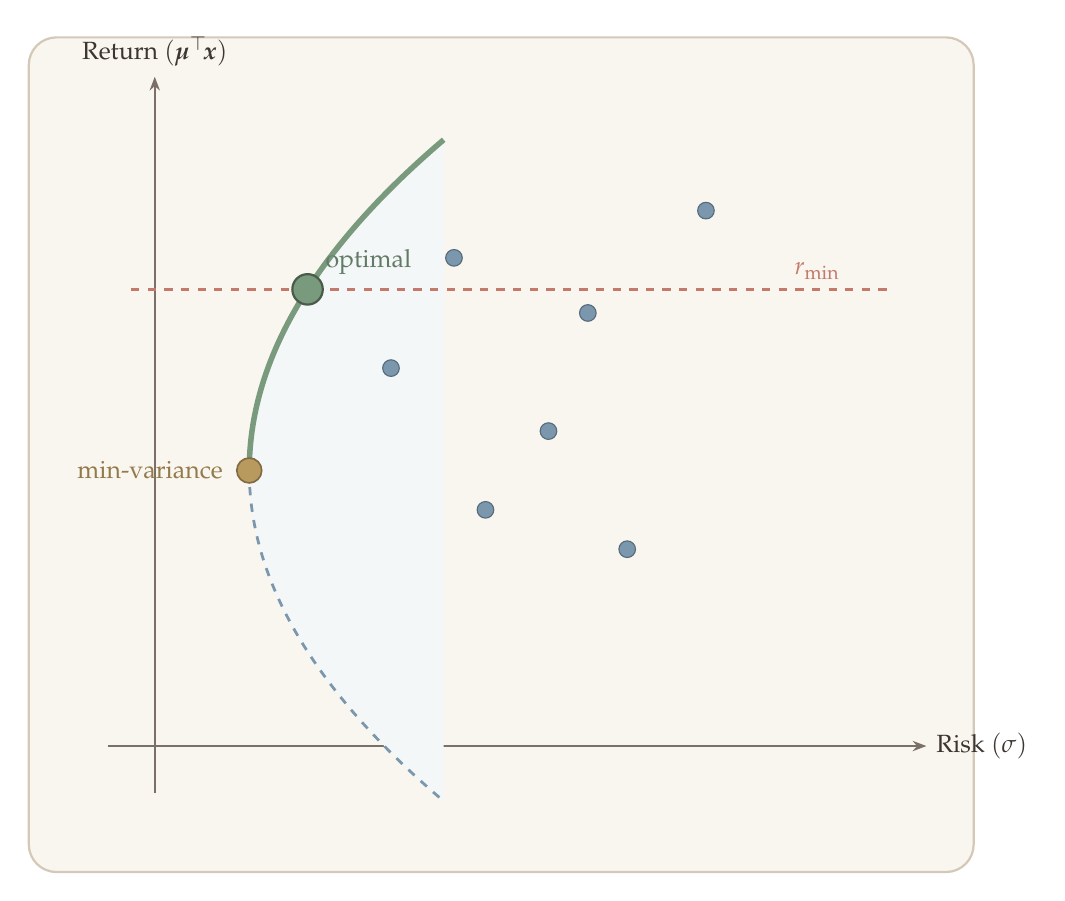
\begin{tikzpicture}[
  >={Stealth[length=3.5mm, width=2.5mm]},
  axis/.style={-{Stealth[length=5pt]}, wmgray, line width=0.6pt},
  lbl/.style={dkbrown, font=\small},
]

% ══════════════════════════════════════════════════════
% Background
% ══════════════════════════════════════════════════════
\fill[cream, rounded corners=10pt] (-1.6,-1.6) rectangle (10.4,9.0);
\draw[border, line width=0.8pt, rounded corners=10pt]
  (-1.6,-1.6) rectangle (10.4,9.0);

% ══════════════════════════════════════════════════════
% Axes
% ══════════════════════════════════════════════════════
\draw[axis] (-0.6,0) -- (9.8,0)
  node[right, lbl] {Risk~$(\sigma)$};
\draw[axis] (0,-0.6) -- (0,8.5)
  node[above, lbl] {Return~$(\boldsymbol{\mu}^\top\!\boldsymbol{x})$};

% ══════════════════════════════════════════════════════
% Parametric bullet (feasible set in risk-return space)
% ══════════════════════════════════════════════════════
% The bullet is parameterised as a sideways parabola:
%   sigma(t) = a*t^2 + sigma_min
%   mu(t)    = mu_min + t
% with t in [-tmax, tmax].
%
% Parameters chosen for good visual proportions:
%   sigma_min = 1.2  (minimum-variance risk)
%   mu_min    = 3.5  (return at minimum-variance portfolio)
%   a         = 0.14
%   tmax      = 4.2

\pgfmathsetmacro{\smin}{1.2}   % minimum risk (x-coordinate of tip)
\pgfmathsetmacro{\mmin}{3.5}   % return at min-variance portfolio
\pgfmathsetmacro{\ascale}{0.14} % curvature
\pgfmathsetmacro{\tmax}{4.2}   % parameter range

% ── Filled feasible region ──────────────────────────
% Upper branch: t from 0 to tmax  (efficient frontier)
% Lower branch: t from 0 to -tmax (inefficient frontier)
% We trace upper then reverse-lower to form a closed path.
\fill[stblue!8]
  plot[variable=\t, domain=0:\tmax, samples=60, smooth]
    ({\ascale*\t*\t + \smin}, {\mmin + \t})
  --
  plot[variable=\t, domain=\tmax:0, samples=60, smooth]
    ({\ascale*\t*\t + \smin}, {\mmin - \t})
  -- cycle;

% ── Inefficient frontier (lower branch, dashed) ─────
\draw[stblue, line width=1pt, dashed]
  plot[variable=\t, domain=0:\tmax, samples=60, smooth]
    ({\ascale*\t*\t + \smin}, {\mmin - \t});

% ── Efficient frontier (upper branch, thick) ─────────
\draw[sage, line width=2pt]
  plot[variable=\t, domain=0:\tmax, samples=60, smooth]
    ({\ascale*\t*\t + \smin}, {\mmin + \t});

% ══════════════════════════════════════════════════════
% Minimum-variance portfolio
% ══════════════════════════════════════════════════════
\fill[rwgold] (\smin, \mmin) circle (4.5pt);
\draw[rwgold!70!black, line width=0.6pt] (\smin, \mmin) circle (4.5pt);
\node[rwgold!80!black, font=\small, anchor=east, xshift=-6pt]
  at (\smin, \mmin) {min-variance};

% ══════════════════════════════════════════════════════
% Target return level r_min
% ══════════════════════════════════════════════════════
\pgfmathsetmacro{\rmin}{5.8}  % target return
\draw[terracotta, line width=1pt, dashed]
  (-0.3, \rmin) -- (9.4, \rmin);
\node[terracotta, font=\small, anchor=south west]
  at (8.0, \rmin) {$r_{\min}$};

% ══════════════════════════════════════════════════════
% Optimal portfolio (intersection of efficient frontier
% with the r_min line)
% ══════════════════════════════════════════════════════
% mu = mmin + t  =>  t = rmin - mmin
\pgfmathsetmacro{\topt}{\rmin - \mmin}
\pgfmathsetmacro{\sopt}{\ascale*\topt*\topt + \smin}

\fill[sage] (\sopt, \rmin) circle (5.5pt);
\draw[sage!60!black, line width=0.8pt] (\sopt, \rmin) circle (5.5pt);
\node[sage!80!black, font=\small, anchor=south west, xshift=3pt, yshift=2pt]
  at (\sopt, \rmin) {optimal};

% ══════════════════════════════════════════════════════
% Individual assets (scattered inside the bullet)
% ══════════════════════════════════════════════════════
% Each (sigma, mu) must satisfy sigma >= a*(mu - mmin)^2 + smin
% i.e., strictly inside the bullet.
\foreach \sx/\sy in {%
  3.0/4.8,%
  4.2/3.0,%
  5.5/5.5,%
  3.8/6.2,%
  6.0/2.5,%
  7.0/6.8,%
  5.0/4.0%
}{
  \fill[stblue] (\sx, \sy) circle (3pt);
  \draw[stblue!70!black, line width=0.4pt] (\sx, \sy) circle (3pt);
}

\end{tikzpicture}
\end{document}
